% Chapter Template

\chapter{Arquitectura de la solución} % Main chapter title

\label{Chapter3} % Change X to a consecutive number; for referencing this chapter elsewhere, use \ref{ChapterX}

%----------------------------------------------------------------------------------------
%  SECTION 1
%----------------------------------------------------------------------------------------

\section{Entrada y salida}

Se asumen tres tipos de entradas que TexToES puede entender.

\begin{itemize}
\item{\textbf{LaTeX}}

Dadas las razones explicadas anteriormente, Latex es un tipo de entrada que nuestra PoC puede entender e interpretar. TexToES asume que la expresión latex está encerrada entre \verb|$| para delimitar el inicio y el fin de ésta.

\textit{Ejemplo}:
$$\verb|$\max(1, 2, 3, 4) = 4$|$$

\item{\textbf{CMathML}}

Como se mencionó, CMathML captura el contenido de la expresión es por eso que se prefiere CMathML antes que PMathML. TexToES asume que la entrada viene dada con su respectiva estructura XML definida por el estándar. Por lo tanto, deberá comenzar con la etiqueta \textbf{<math>}.

\textit{Ejemplo}:
$$\textit{\textbf{<math>}<apply><eq/><ci>a</ci><ci>b</ci></apply>\textbf{</math>}}$$

\item{\textbf{Archivo que contenga expresiones latex}}

TexToES también admite cualquier archivo con extensión \textit{*.txt} que dentro contenga expresiones latex. Se debe cumplir también aquí que las expresiones están encerradas entre \verb|$|.

\end{itemize}

Para cada tipo de entrada obtenemos un texto como tipo de salida que es la representación en lenguaje natural español de la entrada selecta. Para visualizarlo mejor, tenemos el siguiente gráfico:

\begin{figure}[H]
\centering
  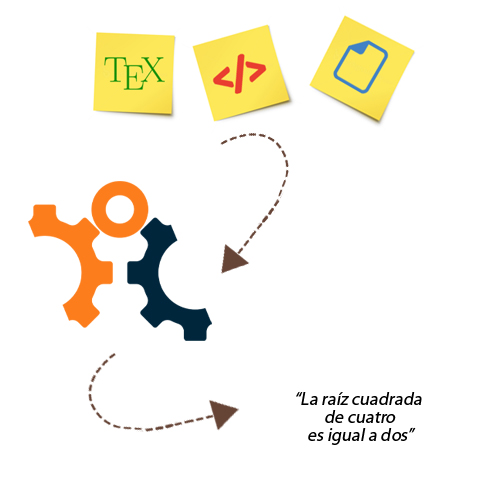
\includegraphics[width=10cm, height=10cm]{Figures/arquitectura-general-textoes}
  \caption[]{Flujo simple de TexToES}
\label{fig:arquitectura}
\end{figure}

Los engranajes representan \textbf{TexToES} y las flechas señalan la dirección del flujo. Más adelante en este documento explicaré con más detalle cómo se compone la PoC.

%----------------------------------------------------------------------------------------
%  SECTION 2
%----------------------------------------------------------------------------------------

\section{A favor de una solución modular}

La manera en que se encaró el desarrollo de TexToEs fue de manera tal que cada componente estuviera aislado y separado del resto.
Llevando a cabo la estrategia \textit{divide y vencerás} fue que se logró programar cada componente por separado, con una interfaz definida para que el resto de los componentes puedan comunicarse a través de ella.

Se decidió distribuir las distintas tareas identificadas en módulos para que se pueda reusar código, para poder adaptar nuevas funcionalidades y la razón más importante es poder utilizar TexToES como un único módulo a la preferencia del usuario o desarrollador.
\\[1cm]

\begin{figure}[H]
\centering
  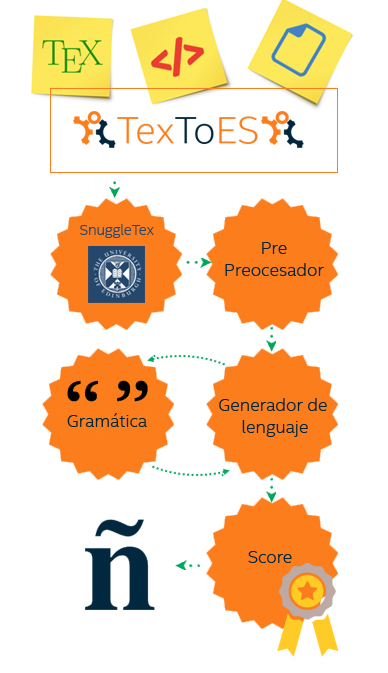
\includegraphics[width=9.22cm, height=16cm]{Figures/detalle-arqui}
  \caption[]{Gráfico de flujo de TexToES}
\label{fig:arquitectura}
\end{figure}

TexToES cuenta con cinco principales módulos los cuales son:

\begin{itemize}
\item Cliente SnuggleTeX: es el cliente que se encarga de comunicarse con el servidor SnuggleTeX, el cliente implementa una sencilla interfaz para hacer y parsear el request que convierte LaTeX a MathML. Esto entra en acción si el usuario quiere verbalizar texto LaTeX.
\item Pre-procesador: Es un simple módulo que pre-procesa el MathML recibido (ya sea por el usuario o el cliente) añadiendo etiquetas y elementos que ayudan al procesamiento del XML, como resultado provee un stack que será manipulado por el verbalizador.
\item Verbalizador o Generador de lenguaje: Se encarga de parsear el stack que representa la fórmula matemática e ir verbalizando cada operador, constructor y constante que encuentre.
\item Gramática: define la gramática utilizada por el Verbalizador.
\item Score: Sistema que evalúa la transcripción obtenida. Indica métricas que muestran el grado de confianza de que tiene el usuario de que su verbalización obtenida esté bien.
\end{itemize}

La combinación de estos módulos forman a TexToES. Cabe mencionar que cada uno de ellos es exportable, i.e. el lector puede importarlos desde su ambiente de desarrollo y los puede usar por separado utilizando su interfaz.

\section{SnuggleTeX y Cliente SnuggleTeX}

SnuggleTeX\cite{3} es una librería Java gratuita y open-source para convertir fragmentos de Latex a XML (usualmente XHTML + MathML). Las funcionalidades principales que SnuggleTex provee son:

\begin{itemize}
\item SnuggleTeX convierte de código matemático simple en LaTeX a MathML, puedes obtener tanto PMathML como CMathML.
\item SnuggleTeX puede convertir el MathML resultante en imágenes (usando la librería JEuclid) y además puede convertir código MathML simple en una mezcla de XHTML y CSS.
\item SnuggleTeX puede tambien enriquecer la salida PMathML que crea, adicionalmente generando CMathML y/o Maxima.
\end{itemize}

Entre otras funcionalidades.

SnuggleTeX es un componente altamente complejo pero que nuestra PoC lo usa como un componente de caja negra, es decir, no conocemos cómo está implementado sólo utilizamos su interfaz y obtenemos sus resultados.

SnuggleTeX es quien se encarga de convertir el código LaTeX\cite{4}, que viene por entrada, a código CMathML para luego alimentar de éste al resto de los componentes para obtener la verbalización.

Dado que ésta herramienta provee un mecanismo de conversión de un tipo a otro, podemos olvidarnos de la creación de un parser en específico para LaTeX que intente traducirlo a MathML, simplemente alimentos a SnuggleTeX con el código Latex que deseemos verbalizar y luego manipulamos su salida en CMathML. Actualmente, ST se encuentra hosteado en un servidor para proyectos académicos donde se puede consumir toda su funcionalidad.

Para poder alimentar y extraer la información de ST, se implementó un cliente HTTP que pueda comunicarse con el servidor que hostea a la herramienta. El cliente conoce dónde está ubicado éste servidor, conoce también, las distintas URIs de cada funcionalidad y también conoce los nombres de los campos con los que ST va a consumir nuestra petición.

Comunicarse con el servidor de ST es básicamente realizar un pedido POST al servidor indicando en el campo \textit{input} el string LaTeX a convertir. Luego el cliente se encarga de parsear su respuesta para obtener el XML asociado, y en caso de que no esté presente devuelve un objeto \textbf{nulo}.

¿Cuáles son los casos en que puede no estar presente el XML asociado?

Para responder ésta pregunta, nos concentramos en las limitaciones de SnuggleTeX. \\
ST tiene un rango limitado de operadores que puede soportar, si el LaTeX que le demos de entrada posee un operador o símbolo que no esté en la siguiente lista no obtendremos un resultados que podamos verbalizar.

La lista es la siguiente:

\begin{figure}[H]
\centering
  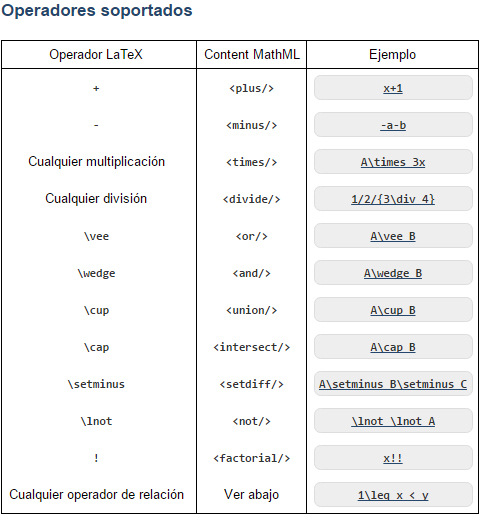
\includegraphics[width=11cm, height=11.84cm]{Figures/opsoportados}
  \caption[]{Operadores soportados por SnuggleTeX}
\label{fig:opsoportados}
\end{figure}

Para los operadores lógicos tenemos:

\begin{figure}[H]
\centering
  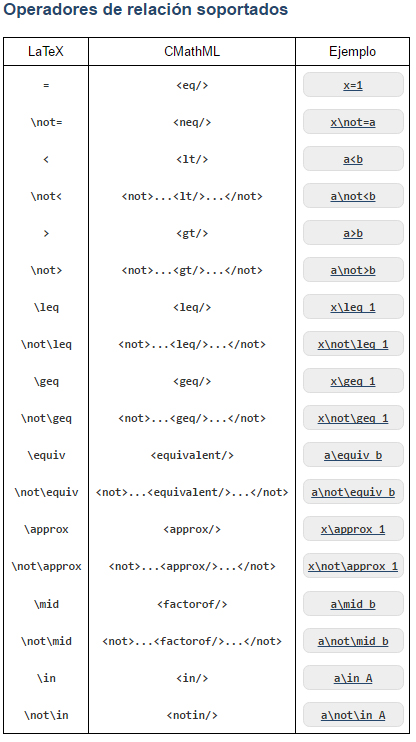
\includegraphics[width=10cm, height=17.84cm]{Figures/reloperatorsoportados}
  \caption[]{Operadores lógicos soportados por SnuggleTeX}
\label{fig:opsoportados}
\end{figure}

También ST puede parsear y dar significado en MathML para funciones pre-definidas.

\begin{tcolorbox}
\verb|\sin \cos \tan \sec \cot \sinh \cosh \lcm \ln \log|\\
\verb|\tanh \sech \csch \coth \arcsin \arccos \max \Re| \\
\verb|\arctan \arcsec \arccsc \arccot \arcsinh \min \det|\\
\verb|\arccosh \arctanh \arcsech \arccsch \gcd \Im \exp \arccoth|
\end{tcolorbox}

Quizás, en algún trabajo futuro, se pueda completar la implementación de SnuggleTeX para aquellos operadores que no estén listados aquí y así agrandar la esfera de acceso de ésta herramienta.

Finalmente, TexToES utiliza ST cuando se alimente nuestra PoC con un string que represente LaTeX. Para los casos en donde directamente dispongamos de una entrada en XML CMathML, ST no estará involucrado en éste escenario.
Luego con el XML CMathML, ya sea provisto por el usuario u obtenido con el cliente de SnuggleTeX, entra en acción el siguiente módulo en el flujo.

\section{Pre-procesador}

El Pre-Procesador (o pre-processor) es el módulo más simple en TexToES pero no menos complejo. Recibe como entrada una cadena de caracteres (string) que represente un XML del tipo CMathML:\\[0.01cm]

\framebox[1.1\width]{\textit{Ejemplo:} <math><apply><eq/><ci>a</ci><ci>b</ci></apply></math>}\\[0.01cm]

Para devolver una pila (stack) con la estructura del árbol XML en una lista utilizando el método de búsqueda \textbf{depth-first}.\\

Éste último método mencionado es un algoritmo muy conocido en el área de Computación que permite recorrer todos los nodos de un árbol de manera ordenada, pero no uniforme. Su funcionamiento consiste en ir expandiendo todos y cada uno de los nodos que va localizando en un camino concreto. Cuando ya no quedan más nodos que visitar en dicho camino, regresa haciendo backtracking, de modo que repite el mismo proceso con cada uno de los hermanos del nodo ya procesado.\\

Se ha utilizado la librería estándar de Python para parsear XML (\textit{xml.etree}).\\

A medida que se recorre el árbol utilizando DF, los elementos del mismo se van apilando utilizando las siguiente reglas de aplicación:

\begin{itemize}
\item \textit{El primer nodo, identificado como "\textbf{math}", se descarta.
\item Por cada nodo etiquetado como "\textbf{apply}" se apila en el stack el string "\textbf{apply}", que es quien indica el inicio de la aplicación de un operador.
\item Por cada nodo etiquetado como "\textbf{end}", se apila en el stack el string "\textbf{end-apply}" similar al anterior, solo que con ésto podemos indicar el fin de la aplicación de la operación.
\item Cada vez que se encuentro un nodo "\textbf{ci}" o "\textbf{cn}" se apila directamente el contenido de su nodo hijo. (Recordemos que ci y cn representan números y variables respectivamente).
\item Cualquier otro caso se apila el nodo sin ninguna alteración.}
\end{itemize}

Cómo habrán notado, la etiqueta "\textbf{end}" no está presente en el string de entrada. Esto es así porque el pre-processor añade esta etiqueta para poder identificar cuando finaliza la aplicación de una operación.
Esta etiqueta custom es una etiqueta dummy su única función es identificar el final de la etiqueta "apply".

Para ello hay un algoritmo simple implementado en este módulo, podemos describir su funcionamiento en la siguiente oración:

\begin{itemize}
\item \textit{Por cada \textbf{</apply>} presente en el texto, añadiré a su izquierda lo siguiente \textbf{<end></end>}. De manera que finalmente quedará reemplazado por <end></end></apply>.}
\end{itemize}

Al finalizar, se entrega una lista (llamada stack) con el contenido del árbol recorrido en DF.\\[0.01cm]

La salida del pre-processor para el ejemplo presentado es la siguiente:\\[0.01cm]

\framebox[1.1\width]{\textit{Salida:} ['apply', 'eq', 'A', 'B', 'end-apply']}\\[0.01cm]


\section{Generador de Lenguaje}

Éste módulo se encarga de verbalizar el stack que recibe desde el pre-processor. Si bien parece simple leyendo esa descripción pero es el módulo más complejo. El módulo provee una manera de generar texto basado en templates (llamado en procesamiento de lenguaje natural como template-based generators\cite{7}).

Procederé a explicar el funcionamiento de éste módulo mediante un ejemplo práctico. Partamos de la siguiente expresión matemática:

$$3x - 2 = 0$$

El cual se puede representar con el siguiente CMathML:

\lstset{language=XML}
\begin{lstlisting}
<math>
   <apply>
       <eq/>
       <apply>
           <minus/>
           <apply>
               <times/>
               <cn>3</cn>
               <ci>x</ci>
           </apply>
           <cn>2</cn>
       </apply>
       <cn>0</cn>
   </apply>
</math>
\end{lstlisting}

Y el stack que obtenemos gracias al pre-processor (y entrada de éste módulo) es el siguiente:\\
\framebox[\width]{ ['apply', 'eq', 'apply', 'minus', 'apply', 'times', '3',
'X', 'end-apply', '2', 'end-apply', '0', 'end-apply'] }

En rangos generales el mecanismo empleado por éste módulo se puede describir con las siguientes reglas:

\begin{enumerate}
\item ¿'apply' está presente en stack?
\begin{enumerate}
  \item si no, terminar.
  \item caso contrario:
  \begin{enumerate}
     \item i es la posición de 'apply' más a la derecha en stack.
     \item j es la posición de 'end-apply' próximo a la derecha de i
     \item creo un stack temporal llamado stack\_temp que contiene el sub array desde i hasta j
     \item obtengo la operación
     \begin{enumerate}
        \item consulto en la gramática por la traducción de la operación
     \end{enumerate}
     \item obtengo su traducción desde la gramática
     \item obtengo la aridad, basándome en la cantidad de operandos en stack\_temp
     \item obtengo la verbalización de stack\_temp
     \item elimino de stack los elementos desde i hasta j y coloco su verbalización
  \end{enumerate}
  \item vuelvo al primer paso
\end{enumerate}
\end{enumerate}

Para el caso planteado podemos ver que 'apply' está presente 3 veces en el stack, por lo que el algoritmo descrito anteriormente se aplicará 3 veces.\\

{\Large \textbf{Primera iteración:}}\\
El elemento 'apply' más a la derecha presente en stack en esta iteración es el que está en la posición 4. Su end-apply próximo está en la posición 8. Por lo tanto el sub stack llamado stack\_temp es el siguiente
$$['apply', 'times', '3', 'X', 'end-apply']$$

Los datos que sé es que la operación en éste stack atómico es \textbf{'times'}, su aridad es \textbf{2} y la gramática (que detallaré más adelante) nos expone que su traducción es \textbf{\$VAR\$ multiplicado por \$VAR\$} donde \$VAR\$ es un símbolo de la gramática que me puede exponer 1 o más transformaciones consecuentes. En éste caso, dado que la aridad es 2, cada \$VAR\$ será reemplazado por los operados (3 y X).

La verbalización consiste simplemente en parsear la traducción desde la gramática y saber colocar desatendidamente los operados en los respectivos \$VAR\$.

Si verbalización finalmente es
$$3 multiplicado por X$$

En el stack original debemos reemplazar todos los elementos stack\_temp presentes en stack por la verbalización obtenida en esta iteración. Finalmente el siguiente es nuestro stack resultante de la primer iteración
$$['apply', 'eq', 'apply', 'minus', '(3 multiplicado por X)', '2', 'end-apply', '0', 'end-apply']$$

{\Large \textbf{Segunda iteración:\\}}
El apply siguiente se encuentra en la posición 2 y su correspondiente end-apply en la posición 6. La operación es \textbf{minus} y su aridad es también \textbf{2}. La gramática nos dice que su traducción es \textbf{\$VAR\$ menos \$VAR\$}. Finalmente su verbalización se corresponde con:
$$((3 multiplicado por X) menos 2)$$

Y el stack resultante es:
$$['apply', 'eq', '((3 multiplicado por X) menos 2)', '0', 'end-apply']$$

{\Large \textbf{Tercera iteración:\\}}
De manera análoga, obtenemos que el resultado final es
$$(((3 multiplicado por X) menos 2) es igual a 0)$$


\subsection{Gramática}

Como se ha mencionado anteriormente, este sistema que busca verbalizar, o traducir, el latex al español tiene su sistema
de generación de lenguaje natural implementado con plantillas, o lo que comúnmente se conoce como template-based generation systems.
TexToES posee una gramática donde mapea las operaciones soportadas (descritas por el operador, o función, en la etiqueta CMathML) con su representación en lenguaje natural. Es simplemente un archivo de configuración donde por cada clave (key) tenemos los operadores y en los valores (value) tenemos su representación en español.\\

La decisión por la que se llevó a cabo la implementación del template es porque se consideró que cada elemento de la etiqueta CMathML tiene una correspondencia uno a uno al español.\\

Por ejemplo, si estamos hablando de \textbf{<plus>} sabemos que estamos hablando de una suma aplicada a dos o más operados. Por lo tanto, en nuestra gramática encontraremos la siguiente línea.\\

\framebox[1.1\width]{ plus = \$VAR\$ más \$VAR\$ }\\

Dónde \$VAR\$ corresponde con símbolos terminales o con otra key dentro de la gramática. Gracias a ésto último podemos describir una suma anidada de números, o simplemente la suma de dos números.\\
Sea $\operatorname{\mathbb{T}}$ todos los elementos que denotan una variable. Por ejemplo, $x,y,f,g \in \operatorname{\mathbb{T}}$.\\
Sea $\operatorname{\mathbb{OP}}$ todos los operadores soportados por TexToES. Por ejemplo, $\textit{suma} \in \operatorname{\mathbb{OP}}$\\

Entonces, VAR en la gramática puede ser involucrar una producción del tipo:
\framebox[1.1\width]{ $VAR = \operatorname{\mathbb{R}}, \operatorname{\mathbb{T}}, \operatorname{\mathbb{OP}}$}\\

La gramática es fácil de extender, por lo tanto, si se quiere añadir soporte para algún operador no soportado, con simplemente describirla en la gramática será suficiente.

Las plantillas o templates son una forma de centralizar la representación del texto origen (source) al texto objetivo (target). Y saca su mayor provecho cuando la representación es uno a uno. Si hubiéramos seguido un approach basado en PMathML en lugar de CMathML, donde para cada PMathML podíamos tener distintas interpretaciones una gramática template-based no nos hubiera ayudado demasiado. Ya que generaríamos, algunas veces, resultados incorrectos o mal interpretados.

La gramática completa puede consultarse en el anexo de éste documento.